\chapter{Grundlagen des Angebots- und Nachfragemodells}

Ein \textbf{Markt} ist ein Mechanismus, durch den Käufer und Verkäufer interagieren um Preise festzulegen und Güter zu handeln. Wir interessieren uns allgemein für die Preisbildung am Markt sowie die Vorgänge, die zur Bildung eines Marktgleichgewichts führen. ~\bigskip

Ein \textbf{Marktgleichgewicht} liegt dann vor, wenn das Angebot der Nachfrage gleicht. Damit ist der Gleichgewichtspreis der Preis $p^*$ für den gilt:
	$$ S(p^*) = D(p^*) $$
Es ist irrelevant, ob hier Gleichheit der Angebots- und Nachfragefunkion oder deren Inversen steht.

\begin{figure*}[!htbp] \centering
	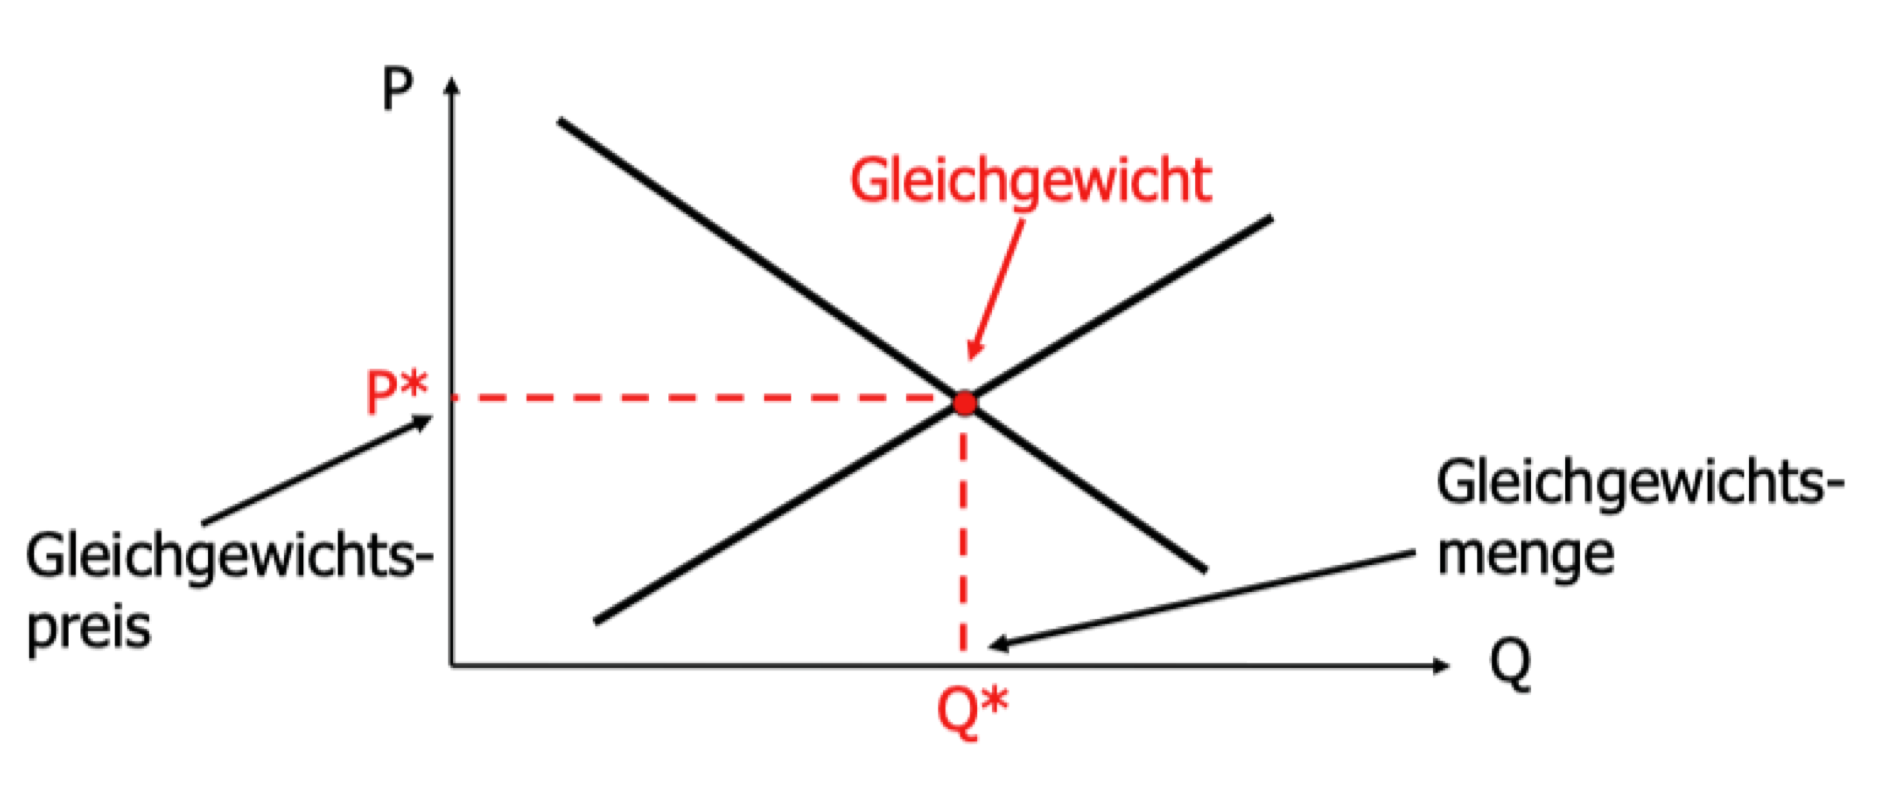
\includegraphics[scale=0.25]{img/marktgleichgewicht}
\end{figure*}

\subsubsection*{Aggregation}

Sind mehrere Anbieter oder Nachfrager auf dem Markt vertreten, so ist die Gesamtmarktnachfrage die horizontale Summe der individuellen (\textbf{Aggregation}).

\begin{kr}[Aggregation der Nachfrage] ~\\
	Bei der Aggregation mehreren Nachfragen $D_i$, die abschnittsweise durch Preise $p_i$ definiert sind, zerteile die einzelnen Nachfragen zuerst nach jedem Abschnittspreis $p_i$. Auf jedem einzelnen Abschnitt ist die aggregierte Nachfrage einfach die Summe der Einzelnachfragen.  
\end{kr}

\begin{kr}[Marktgleichgewicht bei aggregierten Nachfragen] ~\\
	Ist die Nachfrage abschnittsweise auf Preisintervallen $[\underline{p}, \overline{p})$ definiert, berechne auf jeden Abschnitt einzeln den möglichen Gleichgewichtspreis $p^*$. Ist $p^* \in [\underline{p}, \overline{p})$ so ist $p^*$ der tatsächliche Gleichgewichtspreis des aggregierten Zustands, ist allerdings $p^* \notin [\underline{p}, \overline{p})$ fahre mit dem nächsten Abschnitt fort.
\end{kr}~\newpage

\subsubsection*{Elastizitäten}

Wie empfindlich die Nachfrage auf eine Änderung eines Parameters (wie z.B. die Preise oder das Einkommens) reagiert, wird durch die entsprechende \textbf{Elastizität} ausgedrückt:
\begin{itemize}
	\item \textbf{Preiselastizität} $\hat{=}$ prozentuale Änderung der Nachfrage nach Gut $i$ im Verhältnis zur prozentualen Änderung des entsprechenden Preises: 
	$$ \epsilon_{i, p} = \epsilon_D(p_i) = \frac{\partial D}{\partial p_i} \frac{p_i}{D} $$
	Ist $|\epsilon_D| > 1$ so spricht man von einer elastischen Nachfrage, ist $|\epsilon_D| = 1$ von einer einheitselastischen und ist $|\epsilon_d| < 1$ von einer unelastischen Nachfrage.
	\item \textbf{Einkommenselastizität} $\hat{=}$ prozentuale Änderung der Nachfrage im Verhältnis zur prozentualen Änderung des Einkommens: $$ \epsilon_{i, m} = \epsilon_D(m) = \frac{\partial D}{\partial m} \frac{m}{D} $$
	\item \textbf{Kreuzpreiselastizität} $\hat{=}$ prozentuale Änderung der Nachfrage  nach Gut $i$, im Verhältnis zur prozentualen Änderung des Preises eines anderen Guts $j$: 
	$$ \epsilon_{ij} = \epsilon_{D_i}(p_j) = \frac{\partial D_i}{\partial p_j} \frac{p_j}{D_i} $$
	Wenn $\epsilon_{ij} > 0$, dann sind Gut $i$ und $j$ Substitute, und wenn $\epsilon_{ij} < 0$, dann sind Gut $i$ und $J$ Komplemente.
\end{itemize} ~\smallskip

\subsubsection*{Renten}

\begin{figure}[htbp!]
	\begin{minipage}[t]{9cm}\vspace{0pt} ~\\
		Die Differenz zwischen dem, was ein Konsument zu bezahlen bereit wäre (Zahlungsbereitschaft) und dem, was er tatsächlich zahlen muss, ist die \textbf{Konsumentenrente}. Grafisch ist die Konsumentenrente die Fläche unter der inversen Nachfragefunktion zwischen 0 und der nachgefragten Menge $x^*$ abzüglich der Ausgaben.
	\end{minipage}
	\hspace{0.25cm}
	\begin{minipage}[t]{3cm}\vspace{1pt}
		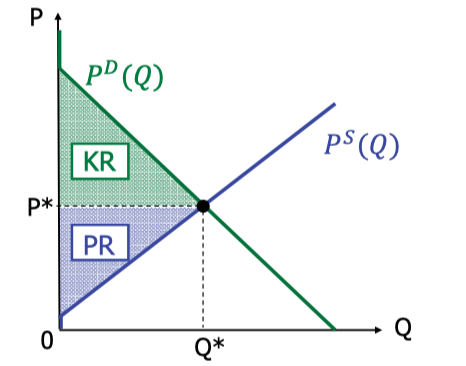
\includegraphics[scale=0.5]{img/krpr}
	\end{minipage}
\end{figure}  ~\smallskip

Die \textbf{Konsumentenrente} wird durch die Fläche oberhalb der inversen Angebotskurve beschrieben. Sie entspricht der Summe der Differenzen zwischen dem niedrigsten Betrag, für welche $x^*$ Einheiten des Gutes angeboten würden, und dem tatsächlichen Preis.  ~\newpage
		
\subsubsection*{Wohlfahrt und Wohlfahrtsverlust}

Die sogenannte Gesamtwohlfahrt ist die Summe aus Konsumenten-, Produzentenrente und möglicher Steuereinnahmen. Sie stellt den Nutzen des sich einstellenden Gleichgewicht dar. Ein Staatseingriff in den Markprozess, wie Höchst- oder Mindestpreise, Subvention und Besteuerung kann zu einem Wohlfahrtsverlust führen. Der Wohlfahrtsverlust ist demnach einfach die Differenz der Wohlfahrt vor und nach dem Eingriff. ~\bigskip

Im Fall der Einführung einer Steuer muss zwischen dem Preis der Nachfrager $p_D$ und dem Preis der Anbieter $p_S$ unterschieden werden. Insbesondere:
\begin{itemize}
	\item wird eine Mengensteuer eingeführt, wird für jede gekaufte Einheit ein Teil des Preises abgeführt. Die Anbieter erhalten lediglich den Verkaufspreis $p_D$ abzüglich der Steuerabgaben, das heißt $p_D = p_S + t$.
	\item wird eine Wertsteuer eingeführt, so wird für jede gekaufte Einheit ein  Anteil des Preises abgeführt. Die Anbieter erhalten lediglich einen um einen Faktor verringerten Verkaufspreis $p_D$, das heißt $p_D = (1 + \tau) \cdot p_S$.
\end{itemize} 
Analog können Subventionen auf die Menge und den Wert des Gutes \enquote{negative} Steuer aufgefasst werden. ~\bigskip

Allerdings muss trotz Steuer auf dem Markt weiterhin ein Gleichgewicht herrschen, das heißt
\begin{equation*}
	D(p^*_D) = S(p^*_S) \tag*{$(*)$}
\end{equation*} 

\begin{kr}[Wohlfahrtsverlust] ~\\
	Bei linearen Angebots- und Nachfragefunktionen können die Konsumenten- und Produzentenrenten, sowie die Steuereinnahmen und der DWL einfach über geometrische Gleichungen berechnet werden (Dreiecksflächen). ~\bigskip
	
	Zuerst ist aus diesem Grund das Gleichgewicht ohne Steuer zu berechnen und dies ergibt $p^*$ und $q*$. Danach mit Steuern berechnet man mittels $(*)$ das neue Gleichgewicht und erhält $p_D^*$ und $p_S^*$. Sei $p_{max}$ zusätzlich der Höchstpreis und $p_{min}$ der Mindestpreis (oft $= 0$) den die Nachfrage bereit ist zu zahlen. 
	
	\begin{minipage}[t]{0.25cm}
		~\
	\end{minipage}
	\begin{minipage}[t]{7.5cm}
		\vspace{0pt} ~\bigskip
		\begin{itemize}
			\item $KR = \frac{1}{2} \cdot (p_{max} - p_D^*) \cdot D(p_D^*)$
			\item $PR = \frac{1}{2} \cdot (p_{S}^* - p_{min}) \cdot D(p_D^*)$
			\item $Steuer = (p_D^* - p_S^*) \cdot D(p_D^*)$
			\item $DWL = \frac{1}{2} \cdot (p_D^* - p_S^*) \cdot (q^* - D(p_D^*))$
		\end{itemize}
	\end{minipage}
	\hspace{0.25cm}
	\begin{minipage}[t]{4.25cm}\vspace{0pt}
		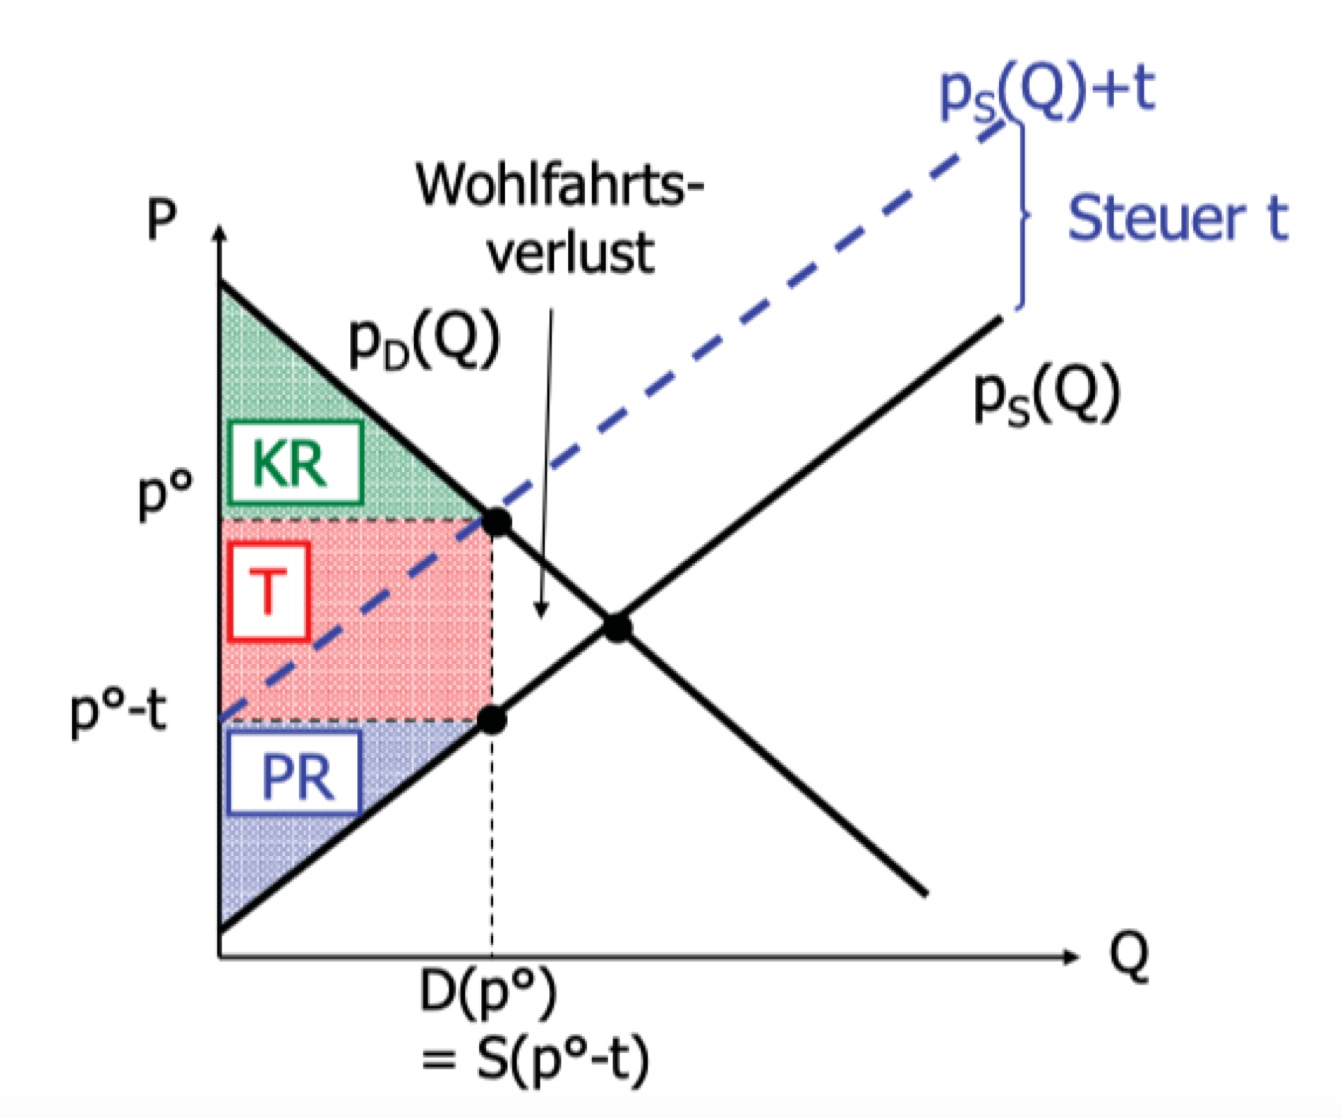
\includegraphics[scale=0.215]{img/dwl}
	\end{minipage}
\end{kr} ~\bigskip

In der Vorlesung wurde auch gezeigt, dass je weniger elastisch die Nachfrage (oder das Angebot) auf Preisänderungen reagieren, desto geringer ist die Zusatzlast durch eine Steuereinführung.